\documentclass[12pt]{article}

% Packages
\usepackage{graphicx}
\usepackage{enumerate}
\usepackage{tabularx}
\usepackage{longtable}
\usepackage{booktabs}
\usepackage{caption}

\usepackage{placeins}
\usepackage{float}
\usepackage{multirow}
\captionsetup[table]{skip=2pt}

\usepackage{geometry}                                       
\geometry{left=2.5cm, right=2.5cm, top=2.5cm, bottom=2.5cm} 

\newcounter{TestCounter}
\setcounter{TestCounter}{0}

\newcounter{ResultCounter}
\setcounter{ResultCounter}{0}

\title{
ClinicFlow
\\\vspace{10mm}
\Large \textbf{Test Report}
\vspace{40mm}
}
\author{ Maxim Vasiliev \#400043983
\and
Susie Yu \#000955758
\and
Karl Knopf \#001437217
\and
Weilin Hu \#001150873
\and
Yunfeng Li \#001335650
}
\date{\today}

% Document adapted from https://github.com/studouglas/GEANT4-GPU/blob/master/Documentation/TestPlan/Test%20Plan.tex 
% and http://itq.ch/pdf/Roadmap%20for%20Testing.pdf


\begin{document}
\pagenumbering{gobble}
\maketitle
\newpage
\tableofcontents
\newpage
\pagenumbering{arabic}
\setlength\parindent{0pt}

\section*{List of Tables}

\begin{center}
\begin{tabular}{cl}
\toprule

\bf Table \# & \bf Title\\\midrule

\ref{Table_Acronyms} & Definitions and Acronyms\\
\ref{PatientInput_unit} & Patient Schedule Input Unit Tests \\
\ref{PatientOutput_unit} & Patient Schedule Output Unit Tests \\
\ref{HealthCareInput_unit}& Health Care Scheduling Input Unit Tests\\
\ref{HealthCareOutput_unit}& Health Care Scheduling Output Unit Tests \\
\ref{ClinicModuleInput_unit}& Module Input Unit Tests \\
\ref{ClinicModuleOutput_unit} &Module Output Unit Tests \\
\ref{SimulationEngine_unit} & Simulation Engine Unit Tests \\

\ref{Login_SystemTests} & Login System Tests \\
\ref{DataStorage_SystemTests} & Database Storage System Tests \\
\ref{DataManipulation_SystemTests} & View, Modify and Delete Data System Tests \\
\ref{ScheduleGeneration_SystemTests} & Schedule Generation System Tests \\
\ref{ViewSchedule_SystemTests} & View Schedule and Modify Schedule System Tests \\
\ref{Usability Tests} & Usability Tests \\
\ref{Performance Tests} & Performance Tests \\
\ref{Table_Schedule} & Testing Schedule \\
\bottomrule
\end{tabular}
\end{center}


\section{Introduction}

\subsection{Introduction}

\subsection{Definitions and Acronyms} 
\begin{center}
\begin{longtable}{>{\raggedright\arraybackslash}p{0.25\textwidth}>{\raggedright\arraybackslash}p{0.65\textwidth}}
\caption{Definitions and Acronyms}\label{Table_Acronyms}\\
\toprule

\bf Acronym & \bf Definition\\\midrule
Provider & Someone who works in the clinic environment (a nurse, doctor, technician)\\\midrule

\bottomrule
\end{longtable}
\end{center}

\section{Unit Testing}
\subsection{Overview}
	As the programs will be written in the Python 3 programming language, we can use the unittest framework. We will define test cases, with inputs and expected outputs and then be able to run this for each module in the system. We have not yet specified the names of each module and the functions contained, but we do have a general idea of what modules we would want and what they should do. These tests will be refined once specific function names and information is known.

\subsection{Patient Scheduling} 
	We intend to have a module in the program that will take in a file containing patients in the clinic, and produce a schedule for them. First we must test if scheduling system can take appropriate inputs. The initial inputs for this test would be that the program has nothing loaded into it currently.
		\subsubsection{Test Inputs}
		\begin{table}[H]
			\centering
			\caption{Unit Tests - \texttt{Patient Schedule-Input}}\label{PatientInput_unit}
			\begin{tabular}{lll}
				\toprule
				\multirow{2}{*}{\bf Test \#}  & \multicolumn{1}{c}{\bf Inputs}\\
				\\\midrule
				\refstepcounter{TestCounter}\arabic{TestCounter}\label{GetPoint_0} & No patient dataset\\
				\\\midrule
				\refstepcounter{TestCounter}\arabic{TestCounter}\label{GetPoint_0} & Sample (valid) patient dataset\\
				\\\midrule
				\refstepcounter{TestCounter}\arabic{TestCounter}\label{GetPoint_0} &Incorrectly formatted patient dataset\\
				\bottomrule
			\end{tabular}
		\end{table}
	% Sample  results table
		\subsubsection{Results}
				\begin{table}[H]
			\centering
			\caption{Unit Tests - \texttt{Patient Schedule-Results March 2017}}\label{PatientInput_unit_results}
			\begin{tabular}{lll}
				\toprule
				\multirow{2}{*}{\bf Test \#}  & \multicolumn{1}{c}{\bf Results}\\
				\\\midrule
				\refstepcounter{ResultCounter}\arabic{ResultCounter}\label{GetPoint_0} &Program Crash, error: can not find patient file\\
				\\\midrule
					\refstepcounter{ResultCounter}\arabic{ResultCounter}\label{GetPoint_0}  & Program loads schedule and  continues to run \\
				\\\midrule
					\refstepcounter{ResultCounter}\arabic{ResultCounter}\label{GetPoint_0}  & Program crash, can not read data from file \\
				\bottomrule
			\end{tabular}
		\end{table}
		
	We must also check the function that will output the
	schedule in a useable form for the rest of the system.
		\subsubsection{Test Inputs}
		\begin{table}[H]
			\centering
			\caption{Unit Tests - \texttt{Patient Schedule-Output}}\label{PatientOutput_unit}
			\begin{tabular}{lll}
				\toprule
				\multirow{2}{*}{\bf Test \#}  & \multicolumn{1}{c}{\bf Inputs}\\
				\\\midrule
				\refstepcounter{TestCounter}\arabic{TestCounter}\label{GetPoint_0} & Sample patient dataset\\
				\\\midrule
				\refstepcounter{TestCounter}\arabic{TestCounter}\label{GetPoint_0} & Sample patient dataset with many repeats\\
				\bottomrule
			\end{tabular}
		\end{table}
	\subsubsection{Results}
	\begin{table}[H]
		\centering
		\caption{Unit Tests - \texttt{Patient Schedule-Output : Results March 2017}}\label{PatientInput_unit_results}
		\begin{tabular}{lll}
			\toprule
			\multirow{2}{*}{\bf Test \#}  & \multicolumn{1}{c}{\bf Results}\\
			\\\midrule
			\refstepcounter{ResultCounter}\arabic{ResultCounter}\label{GetPoint_0} & Output in usable form\\
			\\\midrule
			\refstepcounter{ResultCounter}\arabic{ResultCounter}\label{GetPoint_0}  & Output in usable form \\
			\bottomrule
		\end{tabular}
	\end{table}	
\subsection{Healthcare Worker Scheduling} 
We intend to have a module in the program that will take in a file containing the names and schedule of the providers. It will then generate a schedule object that the simulation can use.
		\subsubsection{Test Inputs}
		\begin{table}[H]
			\centering
			\caption{Unit Tests - \texttt{HealthCare Schedule-Input}}\label{HealthCareInput_unit}
			\begin{tabular}{lll}
				\toprule
				\multirow{2}{*}{\bf Test \#}  & \multicolumn{1}{c}{\bf Inputs}\\
				\\\midrule
				\refstepcounter{TestCounter}\arabic{TestCounter}\label{GetPoint_0} & No health care dataset\\
				\\\midrule
				\refstepcounter{TestCounter}\arabic{TestCounter}\label{GetPoint_0} & Sample health care dataset\\
				\\\midrule
				\refstepcounter{TestCounter}\arabic{TestCounter}\label{GetPoint_0} &Incorrectly formatted health care dataset\\
				\bottomrule
			\end{tabular}
		\end{table}
	\subsubsection{Results}
	\begin{table}[H]
		\centering
		\caption{Unit Tests - \texttt{Health Care Schedule-Results March 2017}}\label{HealthCareInput_unit_results}
		\begin{tabular}{lll}
			\toprule
			\multirow{2}{*}{\bf Test \#}  & \multicolumn{1}{c}{\bf Results}\\
			\\\midrule
			\refstepcounter{ResultCounter}\arabic{ResultCounter}\label{GetPoint_0} &Program Crash, error: can not find health care file\\
			\\\midrule
			\refstepcounter{ResultCounter}\arabic{ResultCounter}\label{GetPoint_0}  & Program loads schedule and  continues to run \\
			\\\midrule
			\refstepcounter{ResultCounter}\arabic{ResultCounter}\label{GetPoint_0}  & Program crash, can not read data from file \\
			\bottomrule
		\end{tabular}
	\end{table}	

%	We must the check the function (or functions) that create the health care schedule object.
%		\subsubsection{Test Inputs}
%		\begin{table}[H]
%			\centering
%			\caption{Unit Tests - \texttt{Health Care Schedule- Scheduling}}\label{HealthCareSchedule_unit}
%			\begin{tabular}{lll}
%				\toprule
%				\multirow{2}{*}{\bf Test \#}  & \multicolumn{1}{c}{\bf Inputs}\\
%				\\\midrule
%				\refstepcounter{TestCounter}\arabic{TestCounter}\label{GetPoint_0} & Sample health care dataset\\
%				\\\midrule
%				\refstepcounter{TestCounter}\arabic{TestCounter}\label{GetPoint_0} & Sample health care dataset with many repeats\\
%				\bottomrule
%			\end{tabular}
%		\end{table}
	
	
		
		We must also check the function that will output the
		schedule in a useable form for the rest of the system.
		\subsubsection{Test Inputs}
		\begin{table}[H]
			\centering
			\caption{Unit Tests - \texttt{Health Care Schedule-Output}}\label{HealthCareOutput_unit}
			\begin{tabular}{lll}
				\toprule
				\multirow{2}{*}{\bf Test \#}  & \multicolumn{1}{c}{\bf Inputs}\\
				\\\midrule
				\refstepcounter{TestCounter}\arabic{TestCounter}\label{GetPoint_0} & Sample (valid) health care dataset\\
				\\\midrule
				\refstepcounter{TestCounter}\arabic{TestCounter}\label{GetPoint_0} & Sample health care dataset with many repeats\\
				\bottomrule
			\end{tabular}
		\end{table}
			\subsubsection{Results}
		\begin{table}[H]
			\centering
			\caption{Unit Tests - \texttt{HealthCare-Output : Results March 2017}}\label{HealthCareOutput_unit_results}
			\begin{tabular}{lll}
				\toprule
				\multirow{2}{*}{\bf Test \#}  & \multicolumn{1}{c}{\bf Results}\\
				\\\midrule
				\refstepcounter{ResultCounter}\arabic{ResultCounter}\label{GetPoint_0} & Output in usable form\\
				\\\midrule
				\refstepcounter{ResultCounter}\arabic{ResultCounter}\label{GetPoint_0}  & Output in usable form \\
				\bottomrule
			\end{tabular}
		\end{table}	

\subsection{Modules} 
Clinics can have a variety of sections (which we shall call modules)  such as Blood taking or xray. Each section can be unique or have multiples. We are going to model each clinic in a data file, which will be read into the system when a simulation is run for that clinic.
		\subsubsection{Test Inputs}
		\begin{table}[H]
			\centering
			\caption{Unit Tests - \texttt{Clinic Modules-Input}}\label{ClinicModuleInput_unit}
			\begin{tabular}{lll}
				\toprule
				\multirow{2}{*}{\bf Test \#}  & \multicolumn{1}{c}{\bf Inputs}\\
				\\\midrule
				\refstepcounter{TestCounter}\arabic{TestCounter}\label{GetPoint_0} & No module dataset\\
				\\\midrule
				\refstepcounter{TestCounter}\arabic{TestCounter}\label{GetPoint_0} & Sample (valid) module dataset\\
				\\\midrule
				\refstepcounter{TestCounter}\arabic{TestCounter}\label{GetPoint_0} &Incorrectly formatted module dataset\\
				\bottomrule
			\end{tabular}
		\end{table}
		\subsubsection{Results}
	\begin{table}[H]
		\centering
		\caption{Unit Tests - \texttt{ClinicModuleInput-Results March 2017}}\label{ClinicModuleInput_unit_results}
		\begin{tabular}{lll}
			\toprule
			\multirow{2}{*}{\bf Test \#}  & \multicolumn{1}{c}{\bf Results}\\
			\\\midrule
			\refstepcounter{ResultCounter}\arabic{ResultCounter}\label{GetPoint_0} &Program Crash, error: can not find clinic file\\
			\\\midrule
			\refstepcounter{ResultCounter}\arabic{ResultCounter}\label{GetPoint_0}  & Program loads clinic file and continues to run \\
			\\\midrule
			\refstepcounter{ResultCounter}\arabic{ResultCounter}\label{GetPoint_0}  & Program crash, can not read data from file \\
			\bottomrule
		\end{tabular}
	\end{table}	
	
	
We must also check that the functions in this module create a valid network of modules for the clinic. 
		\subsubsection{Test Inputs}
		\begin{table}[H]
			\centering
			\caption{Unit Tests - \texttt{Clinic Module-Output}}\label{ClinicModuleOutput_unit}
			\begin{tabular}{lll}
				\toprule
				\multirow{2}{*}{\bf Test \#}  & \multicolumn{1}{c}{\bf Inputs}\\
				\\\midrule
				\refstepcounter{TestCounter}\arabic{TestCounter}\label{GetPoint_0} & Sample (valid) clinic module system with no repeats\\
				\\\midrule
				\refstepcounter{TestCounter}\arabic{TestCounter}\label{GetPoint_0} & Sample (valid) clinic module system with many repeats\\
				\bottomrule
			\end{tabular}
		\end{table}
\subsubsection{Results}
	\begin{table}[H]
		\centering
		\caption{Unit Tests - \texttt{ClinicModule-Output : Results March 2017}}\label{HealthCareOutput_unit_results}
		\begin{tabular}{lll}
			\toprule
			\multirow{2}{*}{\bf Test \#}  & \multicolumn{1}{c}{\bf Results}\\
			\\\midrule
			\refstepcounter{ResultCounter}\arabic{ResultCounter}\label{GetPoint_0} & Output in usable form\\
			\\\midrule
			\refstepcounter{ResultCounter}\arabic{ResultCounter}\label{GetPoint_0}  & Output in usable form \\
			\bottomrule
		\end{tabular}
	\end{table}	
	

\subsection{Simulation Engine} 
The system relies on the simulation engine to generate any results. This module must be able to take in the previous schedules and data, and use that to run a discrete event simulation using those schedules. The pass criteria for this engine should be that it is capable of generating realistic schedules. To do this, we ran data set through the engine and randomly selected patients to check to see if they followed a logical path thorugh the clinic.
		\subsubsection{Test Inputs}
		\begin{table}[H]
			\centering
			\caption{Unit Tests - \texttt{Simulation Engine}}\label{SimulationEngine_unit}
			\begin{tabular}{lll}
				\toprule
				\multirow{2}{*}{\bf Test \#}  & \multicolumn{1}{c}{\bf Inputs}\\
				\\\midrule
				\refstepcounter{TestCounter}\arabic{TestCounter}\label{GetPoint_0} & A dataset that is based on actual clinic data\\
				\bottomrule
			\end{tabular}
		\end{table}
\subsubsection{Results}
\begin{table}[H]
	\centering
	\caption{Unit Tests - \texttt{Simulation Engine : Results March 2017}}\label{HealthCareOutput_unit_results 1}
	\begin{tabular}{lll}
		\toprule
		\multirow{2}{*}{\bf Test \#}  & \multicolumn{1}{c}{\bf Results}\\
		\\\midrule
		\refstepcounter{ResultCounter}\arabic{ResultCounter}\label{GetPoint_0} & Clinic Output made logical sense, results were realistic.\\
		\bottomrule
	\end{tabular}
\end{table}		
	
\begin{table}[H]
	\centering
	\caption{Unit Tests - \texttt{Simulation Engine-Output : Results March 2017}}\label{HealthCareOutput_unit_results 2}
	\begin{tabular}{lllll}
		\toprule
		\multirow{2}{*}{\bf Test \#}  & \multicolumn{1}{c}{\bf Results}\\
		\\\midrule
		Number & Sched App Time & Arrival Time & Departure Time \\
		\midrule
		24 & 09:00:00 AM & 08:05:00 AM & 10:12:00 AM \\
		62 & 8:00:00 AM	& 7:55:00 AM &10:07:00 AM \\
		82 & 2:00:00 PM	& 1:40:00 PM& 3:10:00 PM \\
		87&	8:45:00 AM&	8:30:00 AM&	11:35:00 AM\\
		123& 10:15:00 AM& 9:50:00 AM& 11:40:00 AM\\
		472& 9:30:00 AM& 9:20:00 AM& 12:15:00 PM\\
		588& 1:30:00 PM& 1:10:00 PM& 2:10:00 PM\\
		\bottomrule
	\end{tabular}
\end{table}		


\section{System Testing}
\subsection{Login} 
The purpose of user login is to ensure that only valid users allowed to in access the system. There are two types of account. One is the  administrator account which has full authority to manipulate the data and control all operable functions of the system. Another one is the viewer account which only can view the information.  Testing retrieves the input account and password and match with the account information in an existing database to determine whether the user is valid and what the user can do.
\begin{center}
\begin{longtable}{c>{\raggedright\arraybackslash}p{4.8cm} >{\raggedright\arraybackslash}p{3cm}>{\raggedright\arraybackslash}p{3cm}}
\caption{System Tests: Login}\label{Login_SystemTests}\\
\toprule
\bf \# & \bf Initial State & \bf Inputs & \bf Pass Criteria\\\midrule
\stepcounter{TestCounter}\arabic{TestCounter} 
& Login Page
Empty input field of account and password.
& Empty input of one of the input fields or both. Click login.
& Stay at same page and error message of empty input.
\\\midrule
\stepcounter{TestCounter}\arabic{TestCounter} 
& Login Page
Empty input field of account and password.
& Valid input of account and password of administrator account. Click login.
& Redirect to the main page of the application, and give user full authority of control.
\\\midrule
\stepcounter{TestCounter}\arabic{TestCounter} 
&Login Page
Empty input field of account and password.
& Valid input of account and password of viewer account .
Click login.
& Redirect to the main page of the application, user only allowed to view the data and schedule.
\\\midrule
\stepcounter{TestCounter}\arabic{TestCounter} 
&Login Page
Empty input field of account and password.
& Invalid of account or invalid password.
Click login.
& Stay at the same page and present an error message of the invalid login.
\\\midrule
\stepcounter{TestCounter}\arabic{TestCounter} 
&Application main page
& Click logout.
& Redirect to the login page.
\\\midrule
\bottomrule
\end{longtable}
\end{center}
\subsection{Insertion and Storage of Data} 
The application should allow administrator account user to insert data such as patient procedure, doctor and nurse shift hours and other necessary data into corresponding databases. The testing will compare the inserted data with the data stored in database. There exists a checking module to validate the input values.
\begin{center}
	\begin{longtable}{c>{\raggedright\arraybackslash}p{4.8cm} >{\raggedright\arraybackslash}p{3cm}>{\raggedright\arraybackslash}p{3cm}}
		\caption{System Tests: Data Storage}\label{DataStorage_SystemTests}\\
		\toprule
		\bf \# & \bf Initial State & \bf Inputs & \bf Pass Criteria \\\midrule
		\stepcounter{TestCounter}\arabic{TestCounter} 
		& Application main page, admin account.
		& Click Add Data.
		& Redirect to the Application adding data page.
		\\\midrule
		\stepcounter{TestCounter}\arabic{TestCounter} 
		& Application adding data page.
		& Add the inexistent data to target database with correct data type. Click submit.
		& Stay in same page and all inputs are cleaned. Data appear in the corresponding database.
		\\\midrule
		\stepcounter{TestCounter}\arabic{TestCounter} 
		& Application adding data page.
		& Add the data to target database with incorrect data type or incorrect pattern.
		Click submit.
		& Stay in same page and save valid data. Error messages indicate the invalid inputs.
		\\\midrule
		\stepcounter{TestCounter}\arabic{TestCounter} 
		& Application adding data page.
		& Add the data which already existed in target database. Click submit.
		& Stay in same page and save data. Error message indicates the redundancy of data.
		\\\midrule
		\stepcounter{TestCounter}\arabic{TestCounter} 
		& Application adding data page.
		& Add data which out of domain (such as reservation date in past days) to target database. Click submit.
		& Stay in same page and save data. Error message indicates that the data out of valid range.
		\\\midrule
		\stepcounter{TestCounter}\arabic{TestCounter} 
		& Application main page, viewer account.
		& Click Add Data. 
		& Error message.
		\\\midrule
		\bottomrule
	\end{longtable}
\end{center}
\subsection{View, Modify and Delete Data} 
Administrator account user can view, modify and delete existed data in database. Viewer account user only can read the data in the database.  According to the selection of user, retrieve corresponding database and display the content on user interface. Changes and deletion created by administrator account user should be stored into database. Testing checks whether the application display right data, and  whether the changes synchronize with database. Test the validation of the database when unexpected actions happen.
\begin{center}
	\begin{longtable}{c>{\raggedright\arraybackslash}p{4.8cm} >{\raggedright\arraybackslash}p{3cm}>{\raggedright\arraybackslash}p{3cm}}
		\caption{System Tests: Data Manipulation}\label{DataManipulation_SystemTests}\\
		\toprule
		\bf \# & \bf Initial State & \bf Inputs & \bf Pass Criteria \\\midrule
		\stepcounter{TestCounter}\arabic{TestCounter} 
		& Application main page, admin and viewer account .
		& Click View Data.
		& Redirect to the View Data page.
		\\\midrule
		\stepcounter{TestCounter}\arabic{TestCounter} 
		& Application view data page, admin and viewer account.
		& Select target database, click view.
		& Stay at same page. Display the content of all data from corresponding database.
		\\\midrule
		\stepcounter{TestCounter}\arabic{TestCounter} 
		& Application view data page, admin and view account.
		& Select target database and give specific condition, click view. 
		& Stay at same page. Display the content of target data from corresponding database.
		\\\midrule
		\stepcounter{TestCounter}\arabic{TestCounter} 
		& Application view data page, admin account.
		& Modify the displayed data and change the value by another valid value. Click save.
		& Stay at same page. The value in display area and database have been changed.
		\\\midrule
		\stepcounter{TestCounter}\arabic{TestCounter} 
		& Application view data page, admin account.
		& Modify the displayed data and change the value by invalid value( empty for required value or out of valid range). Click save.
		& Stay at same page, no change happen in displayed data or database. Error messages indicate the unexpected changes.
		\\\midrule
		\stepcounter{TestCounter}\arabic{TestCounter} 
		& Application view data page, admin account.
		& Delete whole one row of data by clicking deletion button at end of the row. Click save. 
		& Stay at same page. The deleted row disappear and the data in database is deleted as well.
		\\\midrule
		\stepcounter{TestCounter}\arabic{TestCounter} 
		& Application view data page, admin account.
		& Delete whole one row of data if the data is expected to use in future (Patient reservation in next few days). Click save.
		& Stay at same page. Pop up a deletion confirmation window. Confirming  the deletion will remove the row from the list. Cancel deletion will save the data.
		\\\midrule
		\stepcounter{TestCounter}\arabic{TestCounter} 
		& Application view data page, viewer account.
		& Modify the displayed data. 
		& Stay at same page. Data is not editable.
		\\\midrule
		\stepcounter{TestCounter}\arabic{TestCounter} 
		& Application view data page, viewer account.
		& Click delete button.
		& Stay at same page. Deletion button does not exist.
		\\\midrule
		\stepcounter{TestCounter}\arabic{TestCounter} 
		& Application view data page, viewer account.
		& Click save.
		& Stay at same page.
		Save button does not exist .
		\\\midrule		
		\bottomrule
	\end{longtable}
\end{center}
\subsection{Schedule Generation} 
The application retrieves data from databases and generates schedules based on back end algorithms. Generating schedule is a critical part in the application, because the Clinic needs accurate schedules without conflicts to maintain the efficiency and minimize the wasting of time for both parties. Thus the generated schedule should be examined carefully by the users. 
\begin{center}
	\begin{longtable}{c>{\raggedright\arraybackslash}p{4.8cm} >{\raggedright\arraybackslash}p{3cm}>{\raggedright\arraybackslash}p{3cm}}
		\caption{System Tests: Schedule Generation}\label{ScheduleGeneration_SystemTests}\\
		\toprule
		\bf \# & \bf Initial State & \bf Inputs & \bf Pass Criteria \\\midrule
		\stepcounter{TestCounter}\arabic{TestCounter} 
		& Application main page, admin account
		& Click generate schedule
		& Redirect to generate page schedule
		\\\midrule
		\stepcounter{TestCounter}\arabic{TestCounter} 
		& Application generate schedule page 
		& Select the type of schedule, click start generating.
		& Create a schedule and display it to user. Saved the schedule into corresponding database.
		\\\midrule
		\stepcounter{TestCounter}\arabic{TestCounter} 
		& Application generate schedule page
		& Insert several data of patients reserve same day, same time, different clinic slots. Select the type of schedule, click start generating.
		& Create a schedule and display it to user. The patients can be issued to same time. Saved the schedule into corresponding database.
		\\\midrule
		\stepcounter{TestCounter}\arabic{TestCounter} 
		& Application generate schedule page
		& Insert several data of patients reserve same day, same time, same clinic slots. Select the type of schedule, click start generating.
		& Create a schedule and display it to user. The patients should be spreaded to different time periods. Saved the schedule into corresponding database.
		\\\midrule
		\stepcounter{TestCounter}\arabic{TestCounter} 
		& Application main page, view account
		& Click generate schedule
		& Stay at same page.
		Generate schedule does not exist.
		\\\midrule
		\bottomrule
	\end{longtable}
\end{center}

\subsection{View Schedule and Modify Schedule}
The application allows administrator account user and viewer account user to view the generated schedules. Administrator account user also has the permission to adjust the schedule. Testing ensures that the changed schedule doesn’t have conflicts. 
\begin{center}
	\begin{longtable}{c>{\raggedright\arraybackslash}p{4.8cm} >{\raggedright\arraybackslash}p{3cm}>{\raggedright\arraybackslash}p{3cm}}
		\caption{System Tests: View Schedule and Modify Schedule}\label{ViewSchedule_SystemTests}\\
		\toprule
		\bf \# & \bf Initial State & \bf Inputs & \bf Pass Criteria \\\midrule
		\stepcounter{TestCounter}\arabic{TestCounter} 
		& Application main page, admin and viewer account.
		& Click view schedule. 
		& Redirect to the view schedule page.
		\\\midrule
		\stepcounter{TestCounter}\arabic{TestCounter} 
		& Application view schedule page, admin and viewer account.
		& Select type and date of the schedule. Click view.
		& Stay at same page. The page displays the existed schedule.
		\\\midrule
		\stepcounter{TestCounter}\arabic{TestCounter} 
		& Application view schedule page, admin account.
		& Click adding button and add a new reserved time into blank area of schedule. Click save.
		& Stay at same page. The new time period is added into schedule.The new schedule is saved into database.
		\\\midrule
		\stepcounter{TestCounter}\arabic{TestCounter} 
		& Application view schedule, page admin account.
		& Click on adding button on a reserved area. Click save 
		& If no error happens , stay at same page. No adding button on a reserved area.
		\\\midrule
		\stepcounter{TestCounter}\arabic{TestCounter} 
		& Application view schedule page, admin account 
		& Click on moving button on a reserved area and choose an empty area. Click save.
		& If no error happens stay at same page. The selected time period is set at new area. The new schedule is saved into database.
		\\\midrule
		\stepcounter{TestCounter}\arabic{TestCounter} 
		& Application view schedule page, admin account 
		& Click on moving button on a reserved area and choose a reserved area. Switch the reservation. Click save.
		& If no error happens, stay at same page. The selected time period  is switched with another one. The new schedule is saved into database.
		\\\midrule
		\stepcounter{TestCounter}\arabic{TestCounter} 
		& Application view schedule page, admin account.
		& Application validates the changes of schedule.
		& Checks on the sequences of procedures in clinic. If adding, moving, and switching violate the the sequence, show error message.
		\\\midrule
		\stepcounter{TestCounter}\arabic{TestCounter} 
		& Application view schedule page, admin account.
		& Click delete button to remove a reservation. Click save. 
		& Pop up a window for deletion confirmation. If continue to delete, remove the reservation. Save the new schedule to database. 
		\\\midrule
		\stepcounter{TestCounter}\arabic{TestCounter} 
		& Application view schedule page, viewer account.
		& Click adding or  click moving or click delete or click save.
		& Stay at same page. No adding button, no moving button, no deletion button, no save button.
		\\\midrule
		\bottomrule
	\end{longtable}
\end{center}


\section{Non-Functional Requirements Testing}

\subsection{Usability}
\begin{center}
	\begin{longtable}{c>{\raggedright\arraybackslash}p{4.8cm} >{\raggedright\arraybackslash}p{3.5cm}>{\raggedright\arraybackslash}p{3cm}>{\raggedright\arraybackslash}p{3cm}}
		\caption{Usability Tests}\label{Usability Tests}\\
		\toprule
		\bf \# & \bf Description & \bf Type & \bf Criterion & Tester(s) \\\midrule
		\stepcounter{TestCounter}\arabic{TestCounter} 
		& We will list the most frequently performed tasks, and the development
		team will use the product to complete them. We count the number of
		mouse clicks.
		& Functional (dynamic, manual)	
		& The average number of mouse clicks should be less than five.    
		& 	Development Team
		\\\midrule
		\stepcounter{TestCounter}\arabic{TestCounter} 
		& We will invite five doctors and five nurses to use our product and
		give them a three minutes demonstration on how to complete a certain
		task. After that, the participants will try to complete the same task.
		& Functional (dynamic, manual)	
		& The participants can complete the same task correctly in three minutes.  
		& 	Testing Team
		\\\midrule
		\stepcounter{TestCounter}\arabic{TestCounter} 
		& We will invite five doctors and five nurses to use our product, but
		we will not give a demonstration on how to complete a certain task.
		Instead, the participants will try to complete it based
		on their previous experience and the hints provided by the application.
		& Functional (dynamic, manual)	
		& The participants can complete the required tasks in five minutes and
		they should encounter fewer than three errors.  
		& 	Testing Team
		\\\midrule
		\bottomrule
	\end{longtable}
\end{center}

\subsection{Performance Testing}
\begin{center}
	\begin{longtable}{c>{\raggedright\arraybackslash}p{4.8cm} >{\raggedright\arraybackslash}p{3.5cm}>{\raggedright\arraybackslash}p{3cm}>{\raggedright\arraybackslash}p{3cm}}
		\caption{Performance Tests}\label{Performance Tests}\\
		\toprule
		\bf \# & \bf Description & \bf Type & \bf Criterion & Tester(s) \\\midrule
		\stepcounter{TestCounter}\arabic{TestCounter} 
		& The development team will use the product to complete the most frequently performed tasks.
		We will calculate the time from the start-up of the application to the completion of the work.
		& Functional (dynamic, manual)	
		& The average time should be less than five minutes.  
		& 	Development Team
		\\\midrule
		\stepcounter{TestCounter}\arabic{TestCounter} 
		& The development team will generate 100000 data points, which is ten times more
		than the expected data points. We will input those data points into our
		application. Next, we will input 100 times more data points into the application.
		& Functional (dynamic, manual)	
		& The application does not crash, and there are no obvious latencies
		(less than 5 seconds for each task) when performing
		the common tasks in the first case. The application can crash in the second case.  
		& 	Development Team
		\\\midrule
		\stepcounter{TestCounter}\arabic{TestCounter} 
		& The development team will generate random data points, which contain problems such as
		incorrect formatting data and illegal characters. We will input those data points into
		our application.
		& Functional (dynamic, manual)	
		& The application does not crash and prompts the users that the input data is not
		correct and how they could correct it.  
		& 	Development Team
		\\\midrule
		\bottomrule
	\end{longtable}
\end{center}

%\section{Automated Testing}

%\subsection{Automated System Testing}

%\subsection{Automated Unit Testing}


\newpage
\section{Collected Samples}

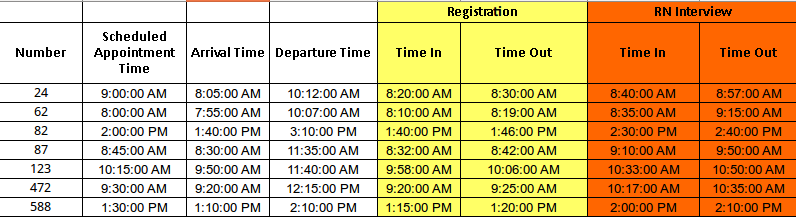
\includegraphics[scale=0.5]{sample1.png}

\quad

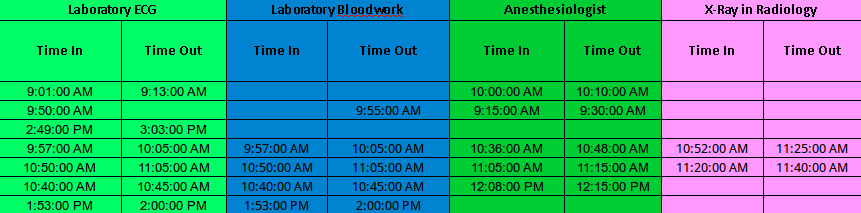
\includegraphics[scale=0.5]{sample2.png}

\subsection{Simulation Results}

u24\\

u24,8:09,arrive,P\\
u24,Registration,8:09,start serivce,P\\
u24,Registration,8:15,leave service,P\\
u24,RNInterview,8:15,start serivce,P\\
u24,RNInterview,8:26,leave service,P\\
u24,LaboratoryECG,8:26,start serivce,P\\
u24,LaboratoryECG,8:35,leave service,P\\
u24,Anesthesiologist,8:50,start serivce,P\\
u24,Anesthesiologist,9:19,leave service,P\\

\quad

u62\\

u62,7:01,arrive,P\\
u62,Registration,7:01,start serivce,P\\
u62,Registration,7:07,leave service,P\\
u62,RNInterview,7:07,start serivce,P\\
u62,RNInterview,7:17,leave service,P\\
u62,LaboratoryECG,7:17,start serivce,P\\
u62,LaboratoryECG,7:26,leave service,P\\
u62,LaboratoryBloodwork,7:26,start serivce,P\\
u62,LaboratoryBloodwork,7:35,leave service,P\\
u62,Anesthesiologist,7:35,start serivce,P\\
u62,Anesthesiologist,7:58,leave service,P\\

\quad

u82\\

u82,13:06,arrive,P\\
u82,Registration,13:06,start serivce,P\\
u82,Registration,13:11,leave service,P\\
u82,RNInterview,13:11,start serivce,P\\
u82,RNInterview,13:22,leave service,P\\
u82,LaboratoryECG,13:22,start serivce,P\\
u82,LaboratoryECG,13:30,leave service,P\\


u87\\

u87,7:53,arrive,P\\
u87,Registration,7:53,start serivce,P\\
u87,Registration,7:59,leave service,P\\
u87,RNInterview,7:59,start serivce,P\\
u87,RNInterview,8:10,leave service,P\\
u87,LaboratoryECG,8:10,start serivce,P\\
u87,LaboratoryECG,8:16,leave service,P\\
u87,LaboratoryBloodwork,8:16,start serivce,P\\
u87,LaboratoryBloodwork,8:23,leave service,P\\
u87,Anesthesiologist,8:23,start serivce,P\\
u87,Anesthesiologist,8:50,leave service,P\\
u87,X-Ray,8:50,start serivce,P\\
u87,X-Ray,9:10,leave service,P\\

\quad

u123\\

u123,9:19,arrive,P\\
u123,Registration,9:19,start serivce,P\\
u123,Registration,9:25,leave service,P\\
u123,RNInterview,9:25,start serivce,P\\
u123,RNInterview,9:44,leave service,P\\
u123,LaboratoryBloodwork,9:44,start serivce,P\\
u123,LaboratoryBloodwork,9:50,leave service,P\\
u123,Anesthesiologist,9:50,start serivce,P\\
u123,Anesthesiologist,10:15,leave service,P\\

(*missing X-Ray part)

\quad

u472\\

u472,8:36,arrive,P\\
u472,Registration,8:36,start serivce,P\\
u472,Registration,8:42,leave service,P\\
u472,RNInterview,8:42,start serivce,P\\
u472,RNInterview,8:59,leave service,P\\
u472,LaboratoryECG,8:59,start serivce,P\\
u472,LaboratoryECG,9:08,leave service,P\\
u472,LaboratoryBloodwork,9:08,start serivce,P\\
u472,LaboratoryBloodwork,9:17,leave service,P\\
u472,Anesthesiologist,9:19,start serivce,P\\
u472,Anesthesiologist,9:43,leave service,P\\

\quad

u588\\

u588,12:32,arrive,P\\
u588,Registration,12:32,start serivce,P\\
u588,Registration,12:39,leave service,P\\
u588,RNInterview,12:39,start serivce,P\\
u588,RNInterview,12:56,leave service,P\\
u588,LaboratoryECG,12:56,start serivce,P\\
u588,LaboratoryECG,13:03,leave service,P\\
u588,LaboratoryBloodwork,13:03,start serivce,P\\
u588,LaboratoryBloodwork,13:11,leave service,P\\



\newpage
\section{Schedule}

\begin{center}
\begin{longtable}{>{\raggedright\arraybackslash}p{0.1\textwidth}>{\raggedright\arraybackslash}p{0.15\textwidth}>{\raggedright\arraybackslash}p{0.55\textwidth}
>{\raggedright\arraybackslash}p{0.1\textwidth}
}

\caption{Testing Schedule}\label{Table_Schedule}\\\toprule

\bf Date Finished & \bf Test Type & \bf Event & \bf Testers\\\toprule

2016-11-20 & Intial Tests & Proof of Concept Demonstration & Development Team \\\midrule
2017-02-12 & Unit Tests & Demonstration Revision 0 & Developement Team \\\midrule
2017-02-12 & System Tests & Demonstration Revision 0 & Developement Team \\\midrule
2017-03-22 & Unit Tests & Test Report Revision 0 & Developement Team \\\midrule
2017-03-22 & System Tests & Test Report Revision 0 & Developement Team \\\midrule
2017-03-22 & Non-Functional Tests & Test Report Revision 0 & Developement Team \\\midrule
2017-04-04 & All Tests & Final Documentation & Developement Team \\\midrule

\bottomrule
\end{longtable}
\end{center}

\end{document}